\section{Evaluation}
\label{sec:eval}
In this section, we introduce the dataset 
and the baseline models that we compare with 
as well as experimental step.
We show the results of our experiments and analyze 
the performance of our model on the evaluation of accuracy
and repetition.


\subsection{Dataset}
CNN/Daily Mail dataset~\cite{HermannKGEKSB15,NallapatiZSGX16,SeeLM17}
\footnote{https://cs.nyu.edu/˜kcho/DMQA/} is a single document dataset,
consisting of 286,817 training pairs,
13,368 validation pairs and 11,487 test pairs.
%\tabref{table:cnn} shows an example pair from training data.
We follow \shortcite{SeeLM17} to preprocess data,
and fill in the blanks with answer named entities.
%We show an example of such pairs in \tabref{tab:gold_a}.

\subsection{Baseline Models}
We introduce five baselines involved in our experiments. Since most works in summarization are RNN-based, to be fair, we transfer techniques from several RNN-based models and build our baselines with convolutional seq2seq architecture.

\textbf{CNN} stands for the original convolutional seq2seq model from \cite{gehring2017convs2s}. Next, we borrow the coverage mechanism from \cite{SeeLM17} to build our \textbf{COV} model as another baseline, where repeatedly
attending to the same locations is penalized in the form of \textit{coverage loss}. In \textbf{ITA}, we incorporate \textit{intra-temporal attention} from \cite{PaulusXS17} into convolutional seq2seq model, which normalizes attention scores using attention history through timestamps. In \textbf{ITDA} model, we further add \textit{intra-decoder attention} mechanism \cite{PaulusXS17}, which normalizes attention using past decoders states. \textbf{TRI} revises beam search in test time in the same way as mentioned in section 2.5 of \cite{PaulusXS17}. In this model, generation of repetitive trigrams is banned during beam search in hope of reducing repetition.

\subsection{Experimental Setup}
\label{sec:expset}
In the following experiments, 
all the competing models have 8 convolutional layers in
both encoders and decoders, with kernel width as 3.
For each convolutional layer, 
we set the hidden vector size as 512 and the embedding size as 256.
To alleviate the overfitting problem,
we add a \textit{dropout} ($p=0.2$) layer for 
all convolutional layers and fully connected layers.

To optimize the proposed model,
we use Nesterov's
accelerated gradient method \cite{SutskeverMDH13} with gradient clipping 0.1 \cite{PascanuMB13}, momentum 0.99,
and learning rate 0.2.
We terminate the training process when the learning rate drops below $10e$-$5$.
We set beam size as 5 for beam search in test time.

To obtain our model with attention filter mechanism and 
sentence-level backtracking decoder, we added the
set $sz$ (in \secref{sec:attf}) as 3.
It depends on the distribution of 
section length in dataset, and nearly 90\% 
of sections with length$>=$3.
We set $c$ (Equation (\ref{eq:s})) as 5,
since the number of overlapped words in target summaries 
is less than 5\%.

Next, we introduce the evaluation metrics in the following experiments:
\begin{enumerate}
\item \textit{ROUGE} scores (F1 score) of the generated
summaries, including ROUGE-1 (R-1), ROUGE-2 (R-2) and
ROUGE-L(R-L)~\cite{rouge-a-package-for-automatic-evaluation-of-summaries}.
%ROUGE-2 is the most popular metric for summarization.

\item \textit{Correctness} (Correct) is the percentage of
\textit{correct} sentences in generated summaries.
Being \textit{correct} means the sentence is free of both grammatical and factual errors. The sentence must be logically implicable from the source document.

\begin{equation}
Correct = \frac{n_{ct}}{N_{all}}
\end{equation}

where $n_{ct}$ and $N_{all}$ denotes respectively
the number of \textit{correct} sentences and all sentences 
in a summary.

\item \textit{Redundancy} (Red) is caused by
repetitive substrings in summary. \textit{Repetitive} means that the sequence appears more than once in a summary. Here we only focus on \textit{repetitive} substrings with length greater or equal to three.
The calculation of redundancy is illustrated in Algorithm \ref{alg:red}.
%Redundancy is different from repeatedness in that it takes into account the length and the number of appearance of repetitive substrings in summary. 

\begin{algorithm}[tb]
\caption{Calculation of redundancy}
\scriptsize
\label{alg:red}
\textbf{Input}: a sentence set $s = {s_{1}, s_{2},...,s_{n}}$\\
%\textbf{Parameter}: Optional list of parameters\\
\textbf{Output}: redundancy percentage $p$
\begin{algorithmic}[1] %[1] enables line numbers
\STATE Let $total$ be the sum of lengths of the sentences in $s$.
\STATE The lengths of longest common substring (LCS) between two sentences from $s$ comprise a length set, $len\_set$.
\STATE Let $n$ be the the largest element in $len\_set$.
\STATE $overlap \leftarrow 0$
\WHILE{$n \geq 3$}
\STATE Find a substring $b$ (with length $n$) that appears the most frequently in $s$.
\STATE Let $k$ be the frequency that $b$ appears in $s$.
\STATE $overlap \leftarrow overlap + k\cdot n$
\STATE Remove every appearance of substring $b$ from sentences in $s$.
\ENDWHILE
\STATE $p \leftarrow overlap/total$
\STATE \textbf{return $p$} 
\end{algorithmic}
\end{algorithm}

\item \textit{Repeatedness}(Rep) consists of N-gram repeatedness
and sentence repeatedness. N-gram repeatedness is
the percentage of repeated N-grams in summary. Sentence
repeatedness is the percentage of repeated sentences.
We use \textit{sim} (Equation (\ref{eq:s})) to estimate
whether sentences are repeated. 
For a sentence, we get $sim$ between it and other sentences
in the same summary. If $sim=1$, it is repeated.
Both repeated N-grams and sentences are repeated units.

\begin{equation}
Rep = \frac{\sum{n_{i}}}{N}
\end{equation}

where $n$ is the number of repeated unit, $i$ 
and $N$ is the number of corresponding N-grams or sentences in a summary.

\end{enumerate}

We use the correctness metric here to complement the ROUGE 
scores because Yao~\shortcite{Yao} showed that the standard ROUGE scores
cannot capture grammatical erros and factual erros. 
Thus, we randomly sample 300 summaries generated by each model, 
and manually inspect their correctness. 
This is a simplified
human-evaluation of summarization, which just
determines whether the sentences in summaries are \textit{correct} or not.
It is easier to accomplish and more reliable than other human-evaluation. 
Compared with repeatedness, redundancy is the comprehensive score 
of repeated unit with length from three to $n$. 

\subsection{Result}
\label{sec:result}

\textbf{Accuracy.} In the experiment, as shown in \tabref{tab:eval_main}, our proposed model ATTF+SBD
outperforms baseline models in ROUGE which shows the
accuracy of the models. Without any operations at testing, our attention
mechanism ATTF has the best score on ROUGE. It denotes
that ATTF is effective to improve the quality of basic CNN seq2seq model.
As for the operations in the test time, both SBD and
TRI have a great improvement on ROUGE score.
It is because that the model can select other words and get more information,
which are adjust to reference summary, from source 
document after reducing repetition.
SBD-1 and SBD-2 are baseline of SBD.
Compared with these two methods, SBD is a little bit lower
but has a higher ROUGE score.
Because any sentences in summary are not distributed by using SBD.
We use SBD as our backtracking decoder in the following experiments.
The ROUGE score of SBD 
is better than TRI on R-1 and R-L, and worse than TRI on R-2. 
The reason is that R-2 and R-L are respectively to evaluate
bigram-overlap and longest common sequence between the reference
summary and generated summary. Corresponding to this, 
SBD select words
based on sentence level while TRI is based on trigrams.
Comparing ATTF+SBD and ATTF+TRI, ATTF+SBD is better. 
Because ATTF filters attention between summary and source document
by each segment in summary, and it need sentence level 
information more than 
ngrams information. 

\begin{table}[th]
	\centering
	\scriptsize
	\begin{tabular}{|l|c|c|c|}
		\hline
		Model &   R-1 & R-2 & R-L \\
		\hline
		CNN &  34.34 & 14.25 & 25.68 \\
		ITA &  34.30 & 14.20 & 25.67 \\
		ITDA & 34.53 & 14.41 &  25.81 \\
	    COV	& 35.85 & 14.80 &  25.95 \\
        TRI* & 36.81 & 15.47 & 26.00 \\
		\hline
		SBD-1* & 34.24 & 14.33 & 24.75 \\
		SBD-2* & 35.88 & 14.83 & 25.15 \\
		SBD* & 37.19 & 15.45 & 26.03 \\
		ATTF & 36.32 & 15.08 & 26.09 \\
		ATTF+TRI* & 37.33 & 15.65 & 26.30 \\
		ATTF+SBD* & \bf 37.69 & \bf 15.82 & \bf 26.47 \\
		\hline
	\end{tabular}
	\caption{ROUGE scores on CNN/Daily Mail dataset. '*' denotes the model with operation at testing.}
	\label{tab:eval_main}
\end{table}

\textbf{Repetition.}
To demonstrate the effectiveness of ATTF and SBD on solving repetition
problem, we compare the repeatedness of summaries generated by
baseline models and our proposed models.
The lower repeatedness reflects better reducing repetition of the model.

\begin{table}[th]
	\centering
	\scriptsize
	\begin{tabular}{|l|c|c|c|c|c|}
		\hline
		Model & 1-gram  & 2-gram & 3-gram & 4-gram & sent \\
		\hline
		Gold & 33.79 & 2.98 & 0.43 & 0.12 & 0.19 \\
		\hline
		CNN &  56.25 & 36.55 & 32.62 & 30.18 & 24.13 \\
		ITA & 54.44 & 34.76 &31.10 & 28.85 & 23.15  \\
		ITDA & 51.18 & 30.64 & 27.14 & 25.04 & 20.19 \\
		COV & 42.18 & 16.77 & 12.95 & 11.17 & 9.05 \\
		ATTF & \bf 34.98 & \bf 8.16 & \bf 5.11 & \bf 4.19 & \bf 2.45 \\
        \hline
		TRI* & 31.91 & 3.17 & \bf 0.0 & \bf 0.0 & \bf 0.01 \\
		SBD* & \bf 29.88 & \bf 2.84 & 0.40 & 0.06 & 0.10 \\
		ATTF+TRI* & 32.0 & 2.94 & \bf 0.0 & \bf 0.0 & 0.09\\
		ATTF+SBD* & 30.83 & 3.71 & 0.74 & 0.13 & 0.14\\
		\hline
	\end{tabular}
	\caption{Repeatedness scores on CNN/Daily Mail dataset. '*' denotes the model with operation
	at testing. The values in table are percentage.}
	\label{tab:eval_repe}
\end{table}

In \tabref{tab:eval_repe}, Gold row stores the repeatedness scores of
reference summaries. ATTF have the lowest
score among models without any operation at test time. 
%It denotes that our model has ability to remember 
%the summarized part of source document by segments in summary.  
%Compared with summaries generated by 
As shown in \figref{fig:attn_maps}, summaries generated by baseline models(\tabref{tab:example} and \tabref{tab:strong_methods})
have repetiton because of attending to same POI of source document. 
ATTF attends to different POI and generates summary 
without repetition as the following:

\fbox{
\parbox{0.9\columnwidth}{
\small{\textbf{ATTF}: ``manchester city are rivalling manchester united and arsenal for defender dayot 
pamecano . the 16-year-old joined in the january transfer window only for 
him to opt to stay in france . ''
}}}

\begin{figure}[th!]
\centering
\subfigure[COV]{
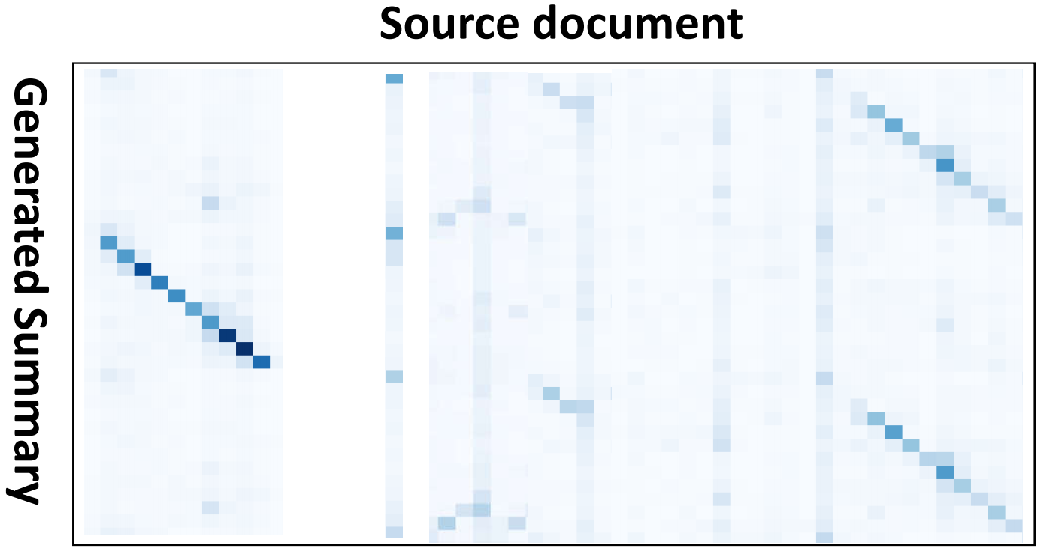
\includegraphics[width=0.45\linewidth]{mapCOV}
}
\quad
\subfigure[ITA]{
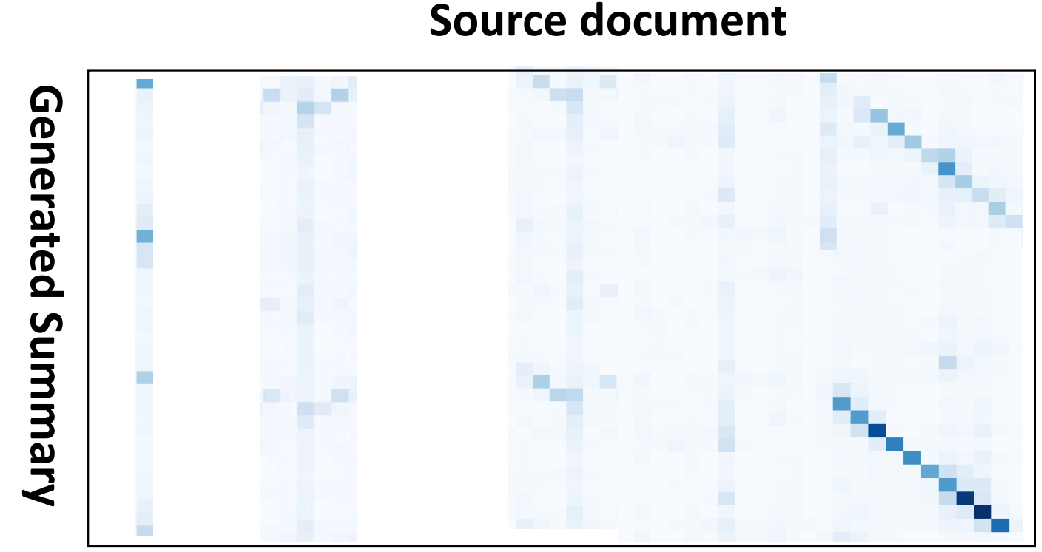
\includegraphics[width=0.45\linewidth]{mapITA}
}
\quad
\subfigure[ITDA]{
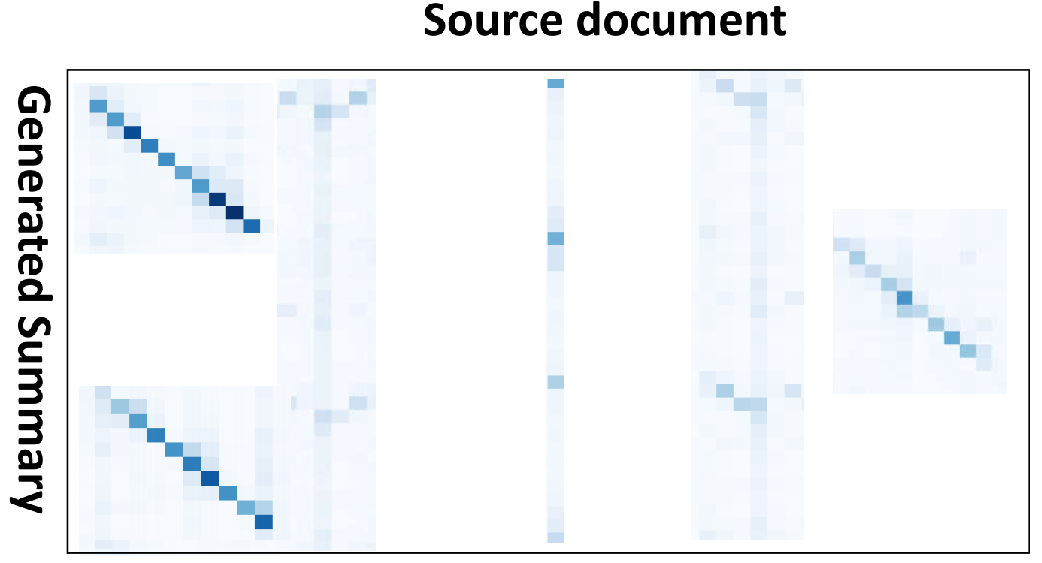
\includegraphics[width=0.45\linewidth]{mapITDA}
}
\quad
\subfigure[ATTF]{
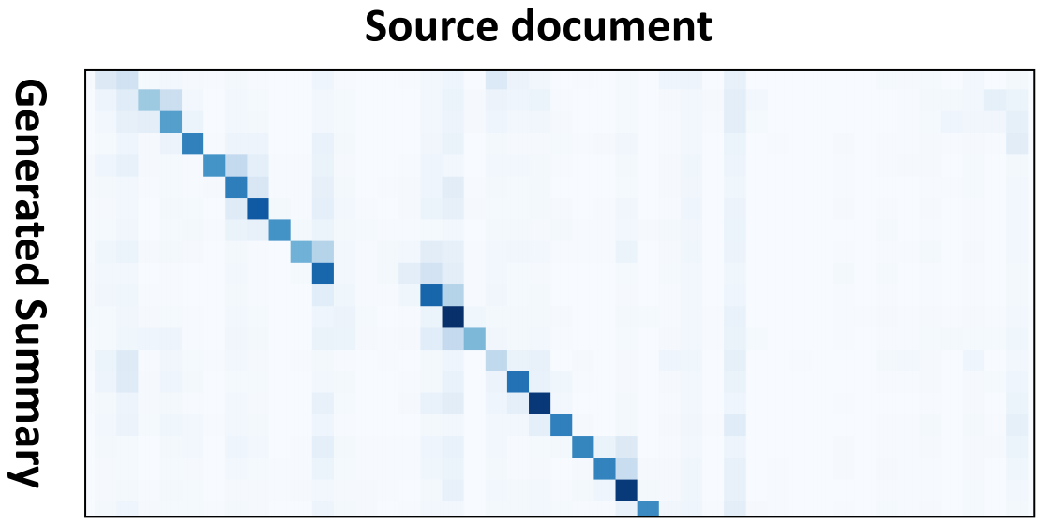
\includegraphics[width=0.45\linewidth]{map2}
}
\caption{Attention distribution for examples in \tabref{tab:strong_methods}}
\label{fig:attn_maps}
\end{figure}

Compared with repeatedness distribution of Gold,
ATTF still generates some repetitive summaries.
The reason is that there are some similar sentences in a source document.
As shown in \tabref{tab:src_rep} and \figref{fig:attn_map3}, repeated sentences
in summary respectively attend to the similar sentences in source document.
SBD is proposed to solve the problem of repetition in source documents.
The repeatedness score of ATTF is reduced after adding SBD.
This shows that SBD is effective.

\begin{table}[th!]
\begin{center}
\scriptsize
\begin{tabular}{lclclclc}%{|p{7cm}|rl|}
%\hline \bf Source document \\
%\hline chelsea 's on loan midfielder oriol romeu goes up against sportsmail 's \\
%       martin ... . the standout fixture in the league on saturday sees leaders \\
%	   chelsea welcome manchester united to stamford bridge , ... \\
%	   chelsea midfielder oriol romeu , \textbf{currently on loan at stuttgart} , predicts \\
%	   the scores for the weekend 's matches . romeu is \textbf{currently on a season-long} \\
%	   \textbf{loan at bundesliga side stuttgart .} \\
%\hline \bf Reference summary \\
%\hline oriol romeu is on a season-long loan at stuttgart from chelsea . the spanish \\
%       midfielder predicts the scores in saturday 's matches . romeu goes \\
%	   head-to-head with sportsmail 's martin keown . \\
\hline \bf Our(Attention Filter)\\
\hline chelsea beat manchester united on saturday . \textit{oriol romeu is currently} \\
       \textit{on a season-long loan at stuttgart . oriol romeu is} \\
	   \textit{currently on a season-long loan at bundesliga side stuttgart .}\\
\hline \bf Our(Attention Filter + Backtracking decoder) \\
\hline chelsea face manchester united in the premier league on saturday . oriol romeu \\
       is currently on loan at stuttgart . \\
\hline
\end{tabular}
\end{center}
\caption{\label{tab:src_rep} Summaries generated by source document with repeatedness. }
\end{table}


\begin{figure}[th!]
\centering
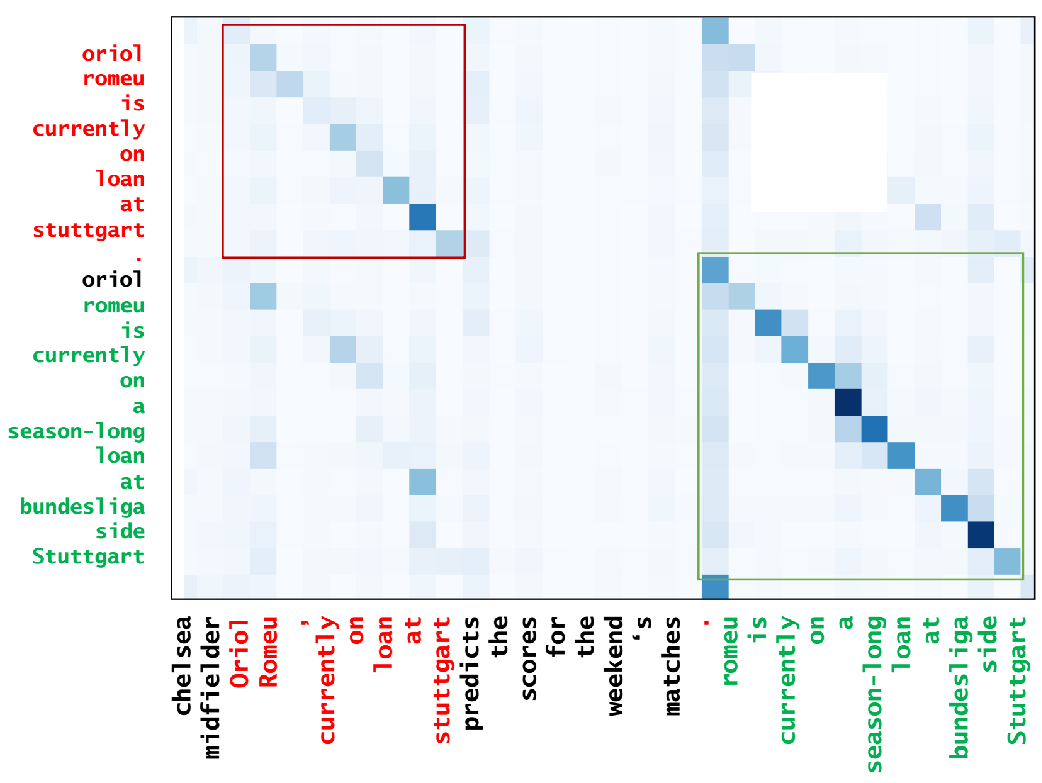
\includegraphics[width=0.9\linewidth]{map3}
\caption{Attention distribution(local) for our attention filter model in \tabref{tab:src_rep}}
\label{fig:attn_map3}
\end{figure}

The repeatedness of models with TRI is the lowest among all of the models, because it
prevents to generate the same trigram at testing. There are no N-grams($N>=3$) repetition
in summaries generated by models with TRI. 
However, according to Gold row, reference summaries have a certain repetition rate.
As reference summaries are standard, we should evaluate the correlation
of repeatedness distribution between
generated summaries and reference summaries. 
We use \figref{fig:reptcor} to illustrate correlations.

\begin{figure}[th!]
\centering
%\includegraphics[width=0.9\linewidth]{corr}
\caption{Repeatedness correlation between different models and Gold summaries.}
\label{fig:repcor}
\end{figure}

We show the correlation of the best baseline(TRI) on repetition 
and our proposed model.
As it shown,
our proposed models have better result, especially ATTF+SBD.
It denotes that ATTF and SBD can respectively solve the problem about
missing POIs in source document and repetition in source document.

\textbf{Human-evaluation.}
In addition, summaries generated by TRI always have grammatical erros
and factual errors, such as TRI row in \tabref{tab:strong_methods}.
In order to demonstrate this, we proposed correctness(seen in \secref{sec:expset}) as
one of our evaluation metric. The correctness scores
are shown in \tabref{tab:eval_cor}. 
TRI has best score on redundancy(Red),which represents the repetiton over N-gram and sentences, but
but lower correctness score than other models.
Besides, the correctness score of ATTF are reduced after adding TRI.
All of our models have correctness score larger than 0.80, and
the correctness score are impoved after adding SBD to ATTF.
It means that SBD can avoid grammatical erros and factual erros.

\begin{table*}[th]
	\centering
	\scriptsize
	\begin{tabular}{|c|c|c|c|c|c|c|c|c|c|c|}
		\hline
	            & Gold & CNN  & ITA & ITDA & COV & TRI & SBD & ATTF & ATTF+TRI & ATTF+SBD \\
		\hline
		Red(\%) & 0.51 & 18.86 & 17.94 & 15.62 & 16.46 & 0.0 & 0.44 & 3.27 & 0.0 & \bf 0.80 \\
		Correct & 1.0 & 0.65 & 0.75 & 0.76 & 0.80 & 0.75 & 0.85 & 0.86 & 0.77 & \bf 0.93 \\
		\hline
	\end{tabular}
	\caption{Redundancy and Correctness scores on CNN/Daily Mail dataset}
	\label{tab:eval_cor}
\end{table*}

\textbf{Speed}.
\begin{table}[th]
\centering
\scriptsize
\begin{tabular}{|l|c|c|c|}
\hline
Model & Time (s) & summaries per sec & tokens per sec \\
\hline
CNN &  346.1 & 30.36 & 1343.46 \\
SBD &  912.8 & 11.51 & 493.68 \\
ATTF & 1121.2 & 9.37 &  401.92 \\
ATTF+SBD & 1332.3 & 7.89 &  349.00 \\
\hline
\end{tabular}
\caption{Testing time, number of generated summaries per second and number of generated tokens per second for different models.}
\label{tab:eval_speed}
\end{table}

\cut{%%%%%%%%%%%%%%%%%%%
\begin{table*}[th]
	\centering
	\scriptsize
	\begin{tabular}{l|c|c|c|c|c|c|c|c}
		\hline
		Model &   1-gram  & 2-gram & 3-gram & 4-gram & 5-gram & sent & Red & Correct \\
		\hline
		Gold & \bf 33.79 & \bf 2.98 & \bf 0.43 & \bf 0.12 & \bf 0.04 & \bf 0.19 & \bf 0.51 & - \\
		\hline
		CNN &  56.25 & 36.55 & 32.62 & 30.18 & 28.07  & 24.13 & 18.86 & 0.65 \\
		ITA & 54.44 & 34.76 &31.10 & 28.85 & 26.89 & 23.15 & 17.94 & 0.75 \\
		ITDA & 51.18 & 30.64 & 27.14 & 25.04 & 23.22 & 20.19 & 15.62 & 0.76 \\
		COV & 42.18 & 16.77 & 12.95 &  & 24.63 & 21.40 & 16.46 & 0.80 \\
		ATTF & 34.98 & 8.16 & 5.11 & 4.19 & 3.65 & 2.45 & 3.27 & 0.86\\
		\hline
		TRI* & 31.91 & 3.17 & - & - & - & 0.01 & - & 0.75 \\
		SBD* & 29.88 & 2.84 & 0.40 & 0.06 & 0.01 & 0.10 & 0.44 & 0.85 \\
		\hline
		ATTF+TRI & 32.0 & 2.94 & - & - & - & 0.09 & - & 0.77 \\
		ATTF+SBD & 30.83 & 3.71 & 0.74 & 0.13 & 0.02 & 0.14  & 0.8 & 0.93 \\
		\hline
	\end{tabular}
	\caption{Repeatedness, Redundancy and Correctness scores on CNN/Daily Mail dataset}
	\label{tab:eval_repe}
\end{table*}
}%%%%%%%%%%%%%%%%%%%


